\begin{figure}[!p]
\centering
\resizebox{\linewidth}{!}{\sffamily
{(a)} \begin{tabular}{c|c|c|c|c|c|c}
\texttt{\#76} (393 nt) & Boltzmann prob. & ensemble defect & struct. distance & energy gap & & \\
``Snowflake 3'' & $p(\vecystar \mid \vecx)$$(\uparrow)$ & \NED$(\vecx, \vecystar)$$(\downarrow)$ & $d(\MFE(\vecx), \vecystar)$$(\downarrow)$ & \DDG$(\vecx, \vecystar)$$(\downarrow)$ & is \MFE & is uMFE \\
\hline
EliteDesign ($N=500$) & \textbf{0.1504} & \textbf{0.0355} & \textbf{0} & \textbf{0.0 kcal/mol} & \textbf{Yes} & \textbf{Yes} \\
SamplingDesign & 0.0444 & 0.0531 & \textbf{0} & \textbf{0.0 kcal/mol} & \textbf{Yes} & \textbf{Yes} \\
\hline
Probability ceiling & 0.7611 & --- & --- & --- & --- & --- \\
\end{tabular}}\\[5pt]
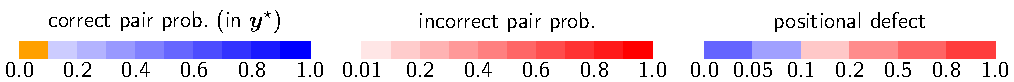
\includegraphics[width=0.9\linewidth]{figures/structures/legend}\\[3pt]
{\sffamily\small
\begin{tabular}{@{}c@{\hspace{0.02\linewidth}}c@{}}
(b) \MFE structure of EliteDesign ($N=500$) ($=$ \vecystar) & (c) \MFE structure of SamplingDesign ($=$ \vecystar) \\[2pt]
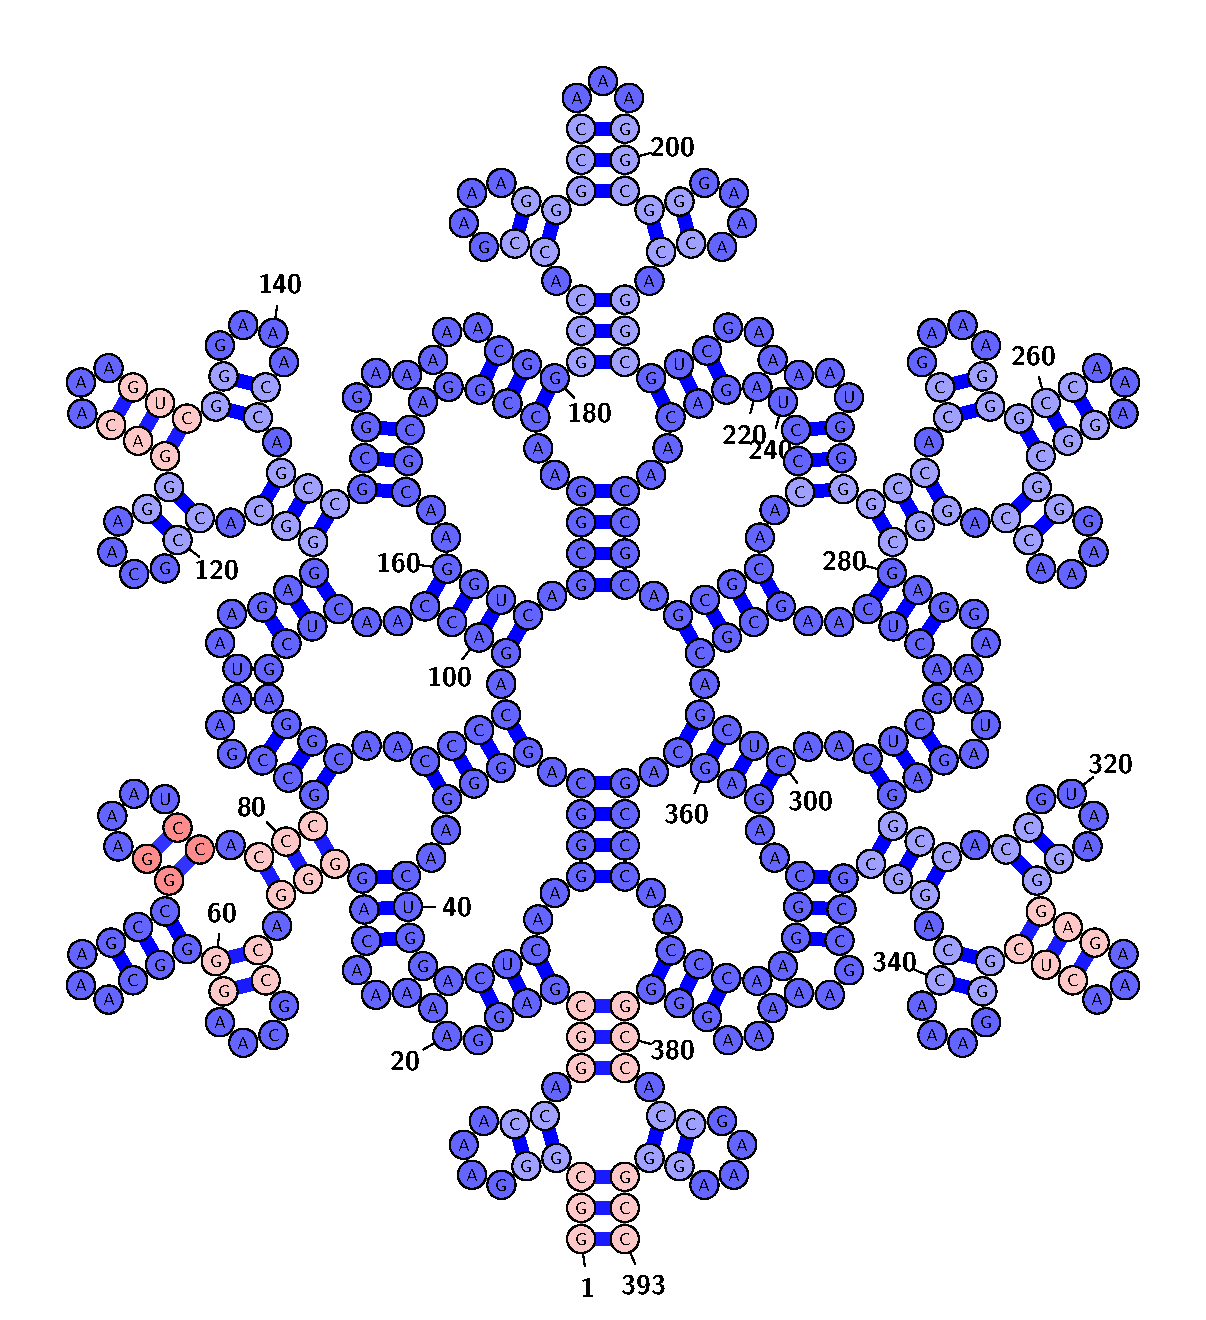
\includegraphics[width=0.49\linewidth]{figures/structures/structure_76_elite} &
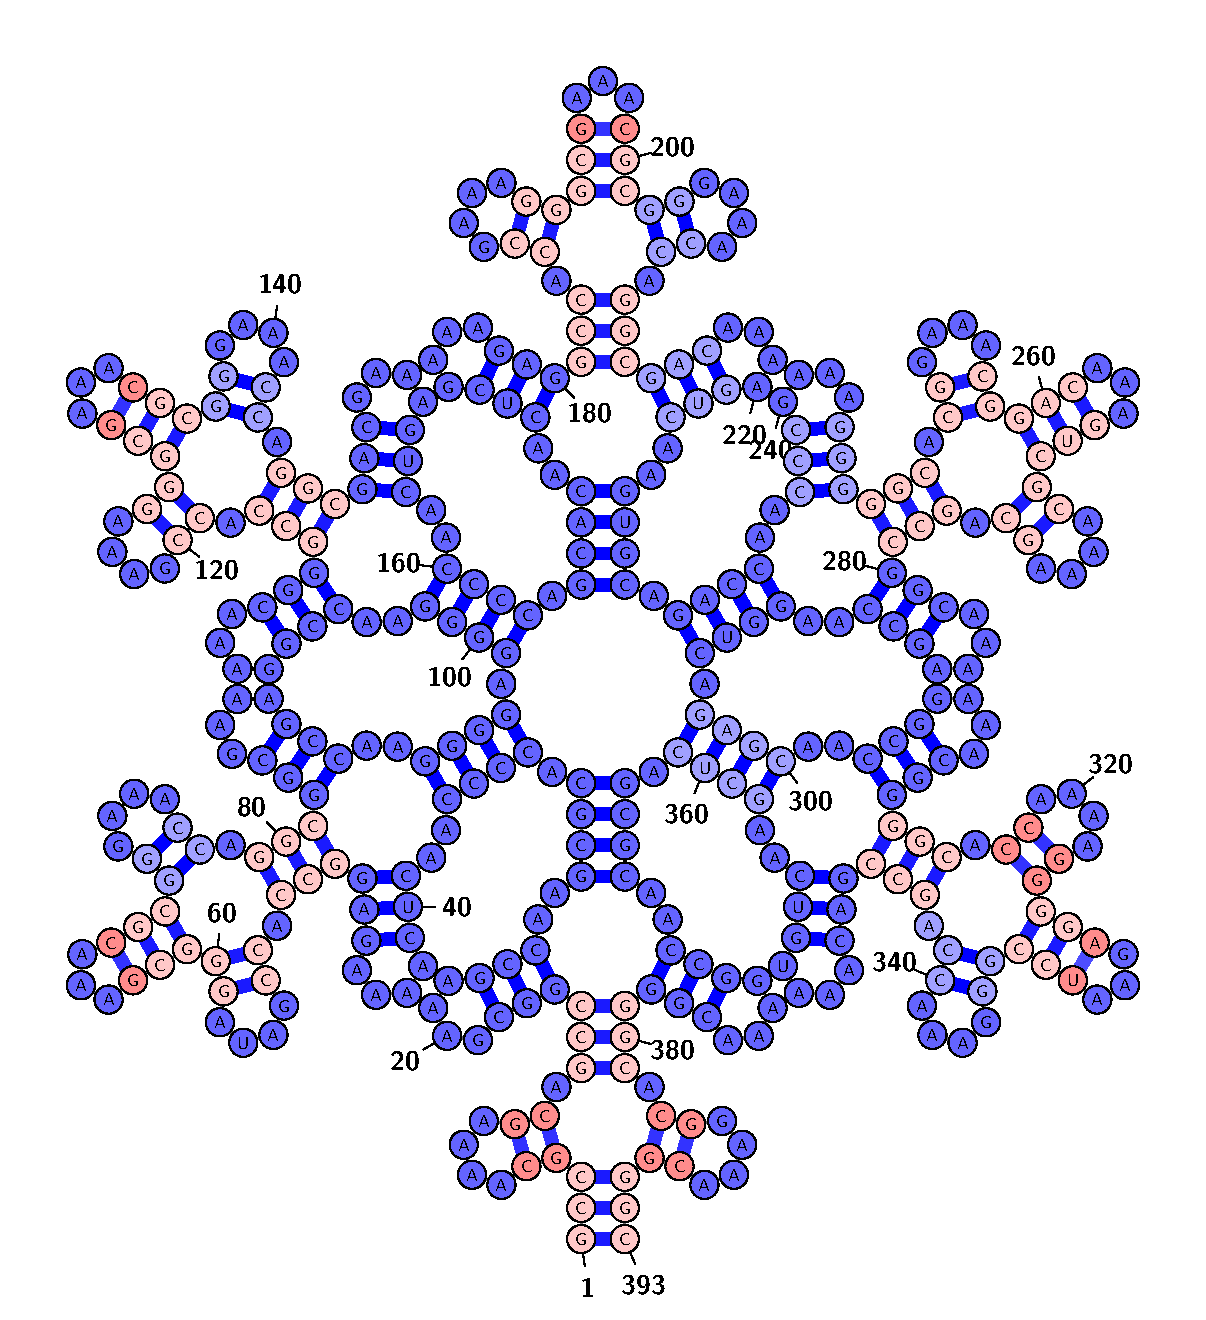
\includegraphics[width=0.49\linewidth]{figures/structures/structure_76_sampling}
\end{tabular}\\[3pt]
\begin{tabular}{@{}c@{\hspace{0.02\linewidth}}c@{}}
(d) Base-pairing probabilities, EliteDesign ($N=500$) & (e) Base-pairing probabilities, SamplingDesign \\[1pt]
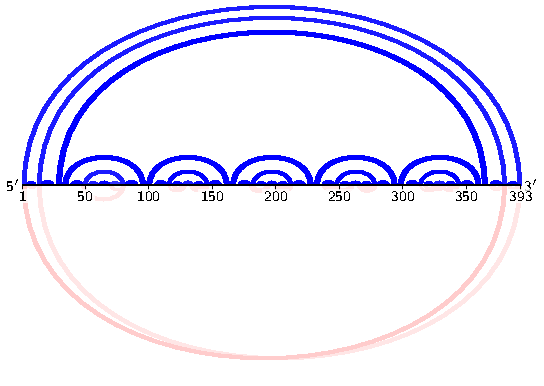
\includegraphics[width=0.49\linewidth]{figures/structures/arcs_76_elite} &
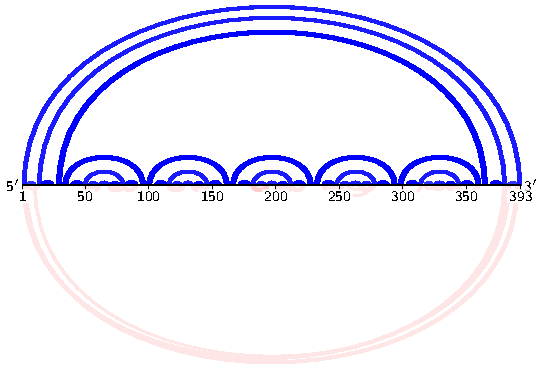
\includegraphics[width=0.49\linewidth]{figures/structures/arcs_76_sampling}
\end{tabular}}
\caption{}
\label{fig:eterna-structure-76}
\end{figure}
